\documentclass[answers]{exam}

% \documentclass[addpoints]{exam}

\usepackage{xeCJK}
\usepackage[utf8]{inputenc}
\usepackage{graphicx}
\usepackage{hyperref}
\usepackage{amsmath}
\usepackage{booktabs}
\usepackage{wrapfig}
\usepackage{color}


\pagestyle{headandfoot}
\firstpageheadrule
\firstpageheader{\textbf{Okayama University}}{\textbf{WANG JING}}{\textbf{Superconductivity Final Exam}}
\runningheader{Okayama University}
{}
{Superconductivity Final Exam}
\runningheadrule
\firstpagefooter{}{Page \quad\thepage\ }{}
\runningfooter{}{Page\quad\thepage\ }{}
%\allowdisplaybreaks


% no box for solutions
% \unframedsolutions

\setlength\linefillheight{.5in}

\renewcommand{\solutiontitle}{\noindent\textbf{Answer:}}
% \renewcommand{\solutiontitle}{\noindent\textbf{解:}\par\noindent}

\renewcommand{\questionlabel}{\thequestion .}
\renewcommand{\thepartno}{\arabic{partno}}
\renewcommand{\partlabel}{\thepartno .}


\begin{document}
\textbf{I. A two-dimensional free-electron gas.}
\vspace{5mm}
\begin{questions}
\question Using the 2-dimensional Schr\"odinger equation, show that the wave function and energy band are :
\begin{gather*}
\psi_{\vec{k}}(\vec{x}) =B \mathrm{e}^{i k_{x} x} \mathrm{e}^{i k_{y} y}\notag \\
E_{\vec{k}} =\frac{\hbar^{2}\left(k_{x}^{2}+k_{y}^{2}\right)}{2 m}\notag   
\end{gather*}
where $m$ is the mass of the electron, $\vec{k} = (k_{x}, k_{y})$ is the wave vector and $B$ is the normalization constant.
\begin{solution}
For  2-D  shr\"odinger Equation:
\begin{align*}
-\frac{\hbar^{2}}{2 m} \nabla^{2} \psi(\vec{r})+V \psi(\vec{r})=E \psi(\vec{r})
\end{align*}
With  V=0 
\begin{align*}
-\frac{\hbar^{2}}{2 m} \nabla^{2} \psi(\vec{r})=E \psi(\vec{r})
\end{align*}
The solution of this equation is travelling plane wave:
\begin{align*}
\psi(\vec{r})=B e^{i \vec{k} \cdot \vec{r}}=B e^{i\left(k_{x} \cdot x+k_{y} \cdot y\right)}
\end{align*}
($e^{-i \vec{k} \cdot \vec{r}}$ term may be absorbed into the direction of $\vec{k}$)\\
And
\begin{align*}
E_{\vec{k}}=\frac{\hbar^{2} k^{2}}{2 m}=\frac{\hbar^{2}\left(k_{x}^{2}+k_{y}^{2}\right)}{2 m}
\end{align*}
\end{solution}

\question By a simple integration over the square of side $L$, find the constant $B$
\begin{solution}
\begin{align*}
\psi(\vec{r})=B e^{i \vec{k} \cdot \vec{r}}=B e^{i\left(k_{x} \cdot x+k_{y} \cdot y\right)}\\
\iint_{0}^{A}\psi(\vec{r}) = 1 \\
\int_{0}^{L}dx\int_{0}^{L}dy|\psi(\vec{r})|^{2} = 1 \\
B^{2} \cdot L^{2} = 1 \\
B = \frac{1}{L}    
\end{align*}
\end{solution}
\newpage
\question Express clearly the allowed values of $\vec{k}$. How many states are in the elementarybox :$\Delta k_{x} \Delta k_{y}=(2 \pi / L)^{2}$?
\begin{solution}
According to PBC,
\begin{align*}
\psi_{k}(x + L, y) = \psi_{k} (x, y),&\quad \psi_{k}(x , y+L) = \psi_{k} (x, y)\\
\text{So for x, we have}\quad\frac{1}{L} e^{i\left(k_{x}\cdot(x+L)+k_{y} \cdot y\right)}&=\frac{1}{L} e^{i\left( k_{x} \cdot x+k_{y} \cdot y\right)} \\
&\Downarrow \\
e^{i k_{x}\cdot  L}&=1 \\
&\Downarrow \\
k_{x}=\frac{2 \pi}{L} n_{x}, \quad n_{x}&=0,\pm 1, \pm 2 \cdots\\
\text{Similarly, for y}\quad k_{y}=\frac{2 \pi}{L} n_{y}, \quad n_{y}&=0,\pm 1, \pm 2 \cdots\\
\text{It is easy to find that:}\quad\Delta k_{x}=\Delta k_{y}=\frac{2 \pi}{L}
\end{align*}
As \textbf{Figure 1} shows, there is only one grid point in each elementary box $\left(\frac{2\pi}{L}\right)^{2}$\\
Of course, if we consider spin, then we have \textbf{two} states in such box.
\end{solution}
\begin{figure}[htbp]
\centering
\begin{minipage}[t]{0.45\textwidth}
\centering
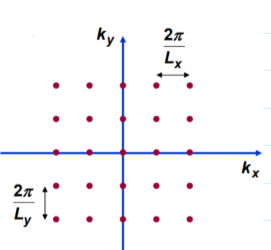
\includegraphics[width=5cm]{Figure/1.png}
\caption{2-D k space}
\end{minipage}
\begin{minipage}[t]{0.45\textwidth}
\centering
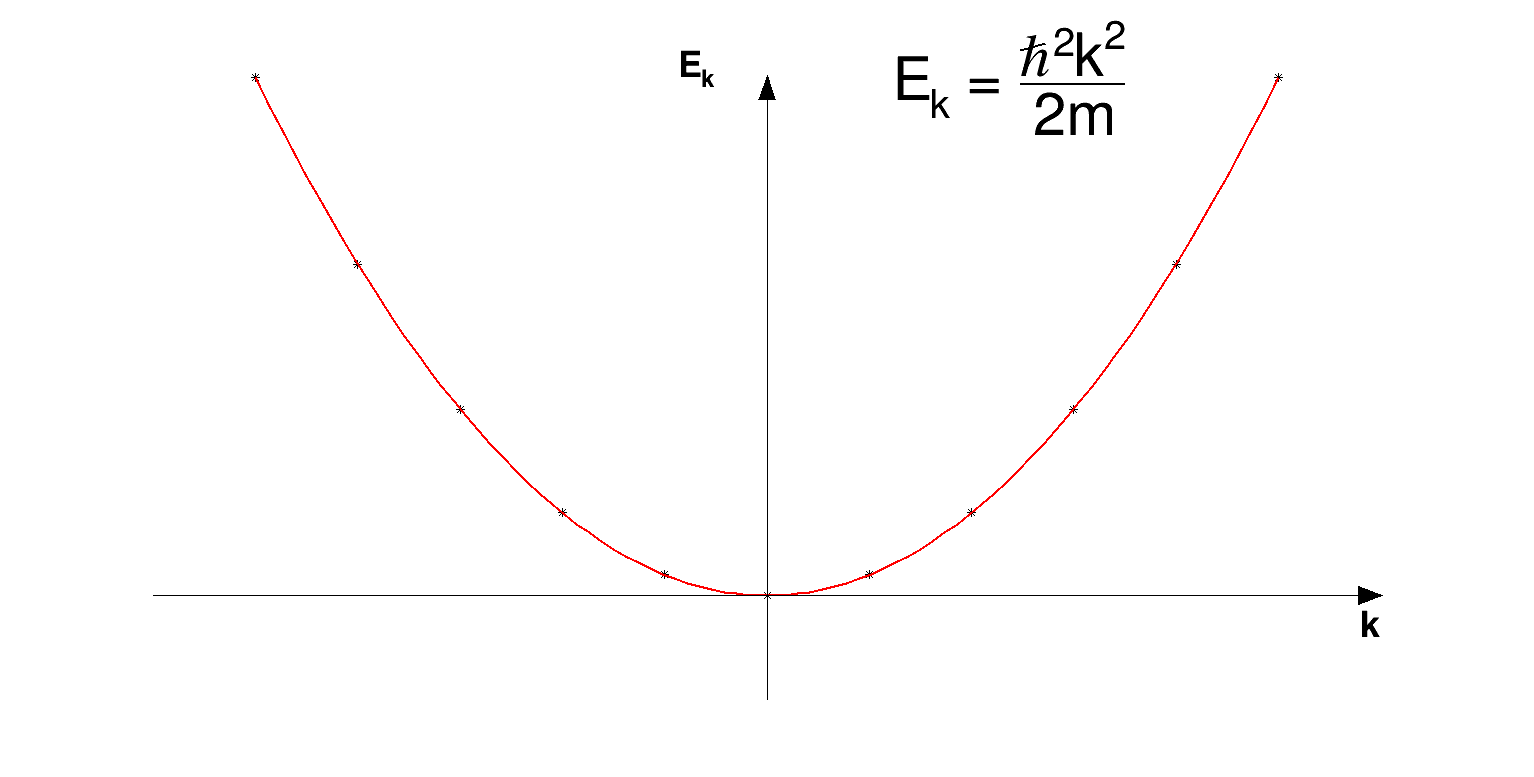
\includegraphics[width=8cm]{Figure/c.png}
\caption{$E_{k}=\frac{\hbar^2k^2}{2m}$}
\end{minipage}
\end{figure}
\question We can also use plane polar coordinates, $\vec{k}=(|\vec{k}|,\varphi)$, so that $k_{x}=|\vec{k}|\cos\varphi$ and $k_{y}=|\vec{k}|\sin\varphi$ in the standard way. Show that the energy band is a parabola as a function of $k=|\vec{k}|$
\begin{solution}
In the polar coordinates:
\begin{align*}
k_{x} &=|k| \cos \varphi \\
k_{y} &=|k| \sin \varphi \\
\text{So, } E_{k} &=\frac{\hbar^{2}\left(\left|k\right|^{2} \cos ^{2} \varphi+|k|^{2} \sin ^{2} \varphi\right)}{2 m}  \\
&=\frac{\hbar^{2} |k|^{2}}{2 m}
\end{align*}
\textbf{Figure 2} shows this relation.
\end{solution}
\newpage
\question  What is the Fermi surface in this 2-dimensional problem ? Please make a drawing in k-space, and mark clearly the occupied and unoccupied regions.
\begin{solution}
The Fermi Surface is when $k_{F}=\sqrt{\frac{2 m E_{F}}{\hbar^{2}}}$, as \textbf{Figure 3} shows, the grid points inside the circle represent the occupied states(yellow part),
while the points outside the circle represent the unoccupied states. 
\end{solution}
\begin{figure}[htbp]
    \centering
    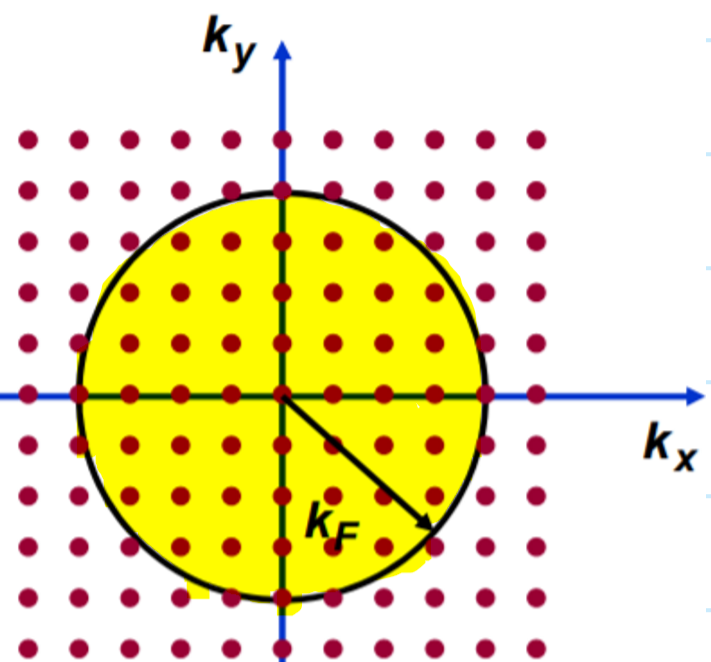
\includegraphics[width=6cm]{Figure/2.png}
\caption{Fermi Surface in 2-D k space}
\end{figure}
\question We must have N electrons confined in our 2-dimensional box. Calculate the electron density $n = \frac{N}{L^{2}}$ using the zero-temperature expression :
\begin{align*}
N=2 \sum_{\vec{k}} \theta\left(k_{F}-|\vec{k}|\right)
\end{align*}
Compare your answer to the analogous law for the 3-dimensional electron gas.
\begin{solution}
Number of electrons is N:
\begin{align*}
N &=2 \sum_{k} \theta\left(k_{F}-|\vec{k}|\right)=2 \iint_{|k|<k_{F}} d n_{x}  d n_{y} \\
&=2 \iint \frac{L d k_{x}}{2 \pi} \cdot \frac{L d k_{ y}}{2 \pi}=\frac{2 A}{(2 \pi)^{2}} \iint d k _{x} d k_{y}  \\
&=\frac{2 A}{(2 \pi)^{2}} \int_{0}^{k_{F}} |k|d|k|\cdot \int_{0}^{2\pi} d\varphi=\frac{2 A}{(2 \pi)^{2}} \cdot \pi\cdot \left|k_{F}\right|^{2} \\
&=\frac{A}{2 \pi}|k_{F}|^{2}\\
\text{So the electron density is }& n =\frac{N}{A}=\frac{|k_{F}|^2}{2\pi}
\end{align*}
In 3-D case, the Fermi Surface is a sphere, so 
\begin{align*}
N&=2 \iiint d n_{x} d n_{y} dn_{z} \\
&=2  \frac{L^{3}}{(2 \pi)^{3}} \iiint d k_{x} d k_{y} d k_{z} \\
&=\frac{2  L^{3}}{(2 \pi)^{3}} \cdot \frac{4}{3} \pi k_{F}^{3} \\
&=\frac{V}{3 \pi^{2}} k_{F}^{3}\\
\text{The electron density is }& n =\frac{N}{V}=\frac{|k_{F}|^3}{3{\pi}^2}
\end{align*}
\end{solution}

\question An important quantity is the density of states, or DOS :
\begin{align*}
    N_{n}(E)=2 \sum_{\vec{k}} \delta\left(E_{\vec{k}}-E\right)
\end{align*}
Do the necessary integration, in the standard fashion, and show that the DOS is a constant $N_{n}(E) = N_{n}$. Polar coordinates should be helpful.
\begin{solution}
\begin{align*}
N_{n}(E)&=2 \sum_{\vec{k}} \delta\left(E_{\vec{k}}-E\right)\\
&=2 \iint d n_{x} d n_{y} \delta\left(E_{k}-E\right) \\
&=2 \left(\frac{L}{2 \pi}\right)^{2} \iint d k x d k y \delta(\cdots) \\
&=2\left(\frac{L}{2 \pi}\right)^{2} \int_{0}^{\infty} k d k \int_{0}^{2 \pi} d \varphi \delta(\cdots)=\frac{A}{\pi} \int_{0}^{\infty} k d k \delta(\cdots) \\
&=\frac{A}{\pi} \int_{0}^{\infty} k \frac{d k}{ {d E_{k}} } {dE_{k}} \delta\left(E_{k}-E\right) \\
&=\frac{A}{\pi} \cdot k \left(\frac{d k}{d E_{k}}\right) _{E_{k}=E} \\
\text{According to }&E_{k}=\frac{\hbar^{2} k^{2}}{2 m}\\
\text{We have }\frac{d E_{k}}{d k}&=\frac{\hbar^{2}}{m} \cdot k \\
&   \colorbox[gray]{0.8}{$k\frac{d k}{d E_{k}}=\frac{m}{\hbar^{2}}$}\\   
\text{So $N_{n}(E)$ is }&=\frac{Am}{\pi\hbar^{2}} \\
\text{And DOS is thus }\frac{N_{n}(E)}{A}&=\frac{m}{\pi\hbar^2}=cte.\\
\end{align*} 
\end{solution}

\question As shown in the figure above (right panel), the energy band $E_{k}$ is directly visible in the ARPES intensity as a function of the parallel wave vector. From
the experimental curve, please give an estimate of the Fermi wave-vector $k_{F}$ and the Fermi energy $E_{F}$.
\begin{figure}[t]
\centering
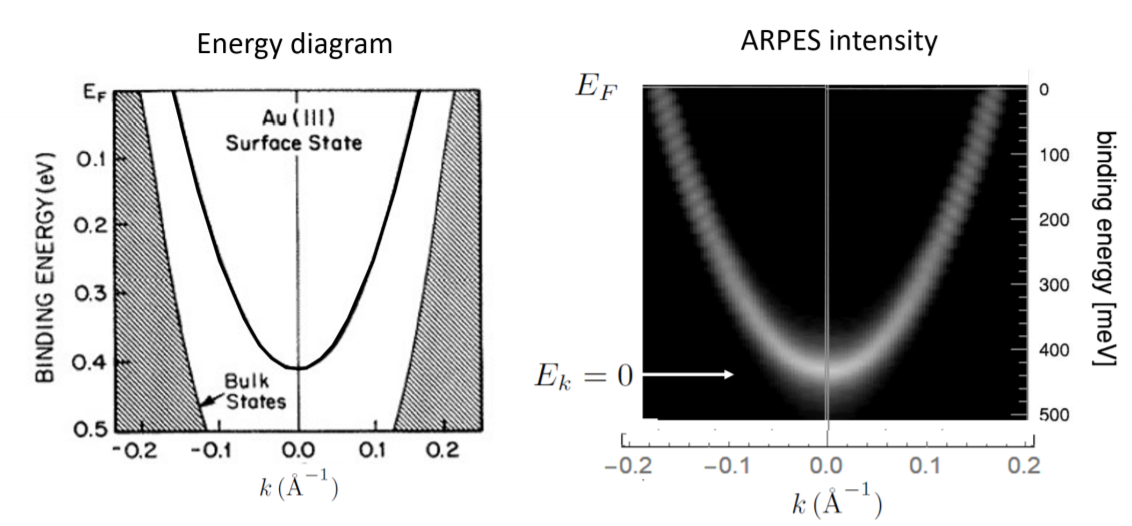
\includegraphics[width=15cm]{Figure/4.png}
\caption{Au(111) ARPES spectrum}
\end{figure}
\begin{solution}
The $k_{F}$ is around 0.16\AA$^{-1}$ , according to $E_{F}=\frac{\hbar^{2} k_{F}^{2}}{2 m}$ , $E_{F}=0.1eV$
\end{solution}




\question Use your expression for the electron density n to estimate it using the experimental value for $k_{F}$ . One decimal precision is enough and express n in both
$m^{-2}$ and \AA$^{-2}$ units. If the distance between two gold atoms is $\sim$ 3\AA, how
many electrons are there per surface unit cell (the lattice is triangular) ?
\begin{solution}
The electron density is $ n =\frac{|k_{F}|^2}{2\pi}$ , $k_{F}=0.16\text{\AA}^{-1}$, so $n=4.1\times10^{-3}\text{\AA}^{-2}=4.1\times 10^{17}m^{-2}$\\
The triangular area is $\frac{\sqrt{3}}{4}r^2=\frac{9\sqrt{3}}{4}\text{\AA}^{-2}$, number of electrons in this unit cell is 0.016.
\end{solution}



\question  Such an electron gas could indeed be superconducting, but the weak coupling
with phonons and low Fermi-level DOS are not favorable. However, suppose
that 0.1\% of the electrons could become Cooper pairs in the superconducting
state. Using the present study, estimate the predicted energy gap in a BCS
model and the corresponding critical temperature $T_{c}$. (We recall that the
number of Cooper pairs is : $N_{n}(E_{F}) \Delta_{0}/2$.)
\begin{solution}
Number of Cooper pairs is $\frac{N_{n}(E_{F})\Delta_{0}}{2}$ , so we have:
\begin{align*}
\frac{N_{n}(E_{F})\Delta_{0}}{2} &= 0.016\times0.1\%\\
\Delta_{0} &= 7.87\times10^{-4}eV \\
\colorbox[gray]{0.8}{$1eV \rightarrow 10^{4}K$} \\
\text{So citical temperature is } T_{c}&=7.87\times10^{-4}eV \approx 7.87K
\end{align*}

\end{solution}

\vspace{5mm}
\textbf{II. The BCS effective Hamiltonian.}
\vspace{5mm}
\question Starting from 
$\tilde{H}_{e f f}=\left(\begin{array}{cc}
    \varepsilon_{k} & -\Delta_{k} \\
    -\Delta_{k}^{*} & -\varepsilon_{k}
    \end{array}\right)$
find the two eigenvalues $E_{k}^{+},E_{k}^{-}$ (Let us consider only $\Delta k$ is real.)
\begin{solution}
In the BCS 'mean-field' approximation, we showed that the electron/hole operators satisfy the simultaneous equations :
\begin{align*}
i \hbar \frac{d}{d t}\left(a_{k \uparrow}\right) &=\varepsilon_{k} a_{k \uparrow}-\Delta_{k} a_{-k \downarrow}^{\dagger} \\
i \hbar \frac{d}{d t}\left(a_{-k \downarrow}^{\dagger}\right) &=-\varepsilon_{k} a_{-k \downarrow}^{\dagger}-\Delta_{k}^{*} a_{k \uparrow}
\end{align*}
We can rewrite it into matrix form or say \textbf{Nambu Formalism}:
\begin{align*}
i \hbar \frac{d}{d t}\left(\begin{array}{l}a_{k \uparrow } \\a_{-k\downarrow }^{\dagger }\end{array}\right)&=\left(\begin{array}{cc}
\varepsilon_{k} & -\Delta k \\
-\Delta{k}^{*} & -\varepsilon_{k}
\end{array}\right)\left(\begin{array}{c}
a_{k \uparrow } \\
a_{-k\downarrow }^{\dagger }
\end{array}\right) 
\end{align*}
In order to diagonalize the matrix $\left(\begin{array}{cc}
\varepsilon_{k} & -\Delta k \\
-\Delta{k}^{*} & -\varepsilon_{k}
\end{array}\right)$ and make it become the eignfunction:
\begin{align*}
i \hbar \frac{d \tilde{\psi}}{d t}&=\tilde{H}_{e f f} \tilde{\psi}
\end{align*}
We introduce the \textbf{Bogoliubov Transformation}, by which we can transfer the eigenfunction to a quasiparticle's eigenfunction with eigenvector$\left(\begin{array}{c}\gamma^{+} \\\gamma^{-}\end{array}\right)$ and eigenvalues $\tilde{{H}_{eff}}$.\\
First, we calculate the eignvalues(energy):
\begin{align*}
\left(E_{k}-\tilde {H}_{eff}\right)\left(\begin{array}{c}
u \\
v
\end{array}\right)=\left(\begin{array}{cc}
E_{k}-\varepsilon_{k} & +\Delta_{k} \\
+\Delta_{k}^{*} & E_{k} +\varepsilon _{k}
\end{array}\right)\left(\begin{array}{c}
u \\
v
\end{array}\right)=0
\end{align*}
It gives an obvious solution:$E_{k}=\sqrt{\Delta_{k}^{2}+\varepsilon_{k}^{2}}$, so
\begin{align*}
E_{k}^{\pm}=\pm\sqrt{\Delta_{k}^{2}+\varepsilon_{k}^{2}}
\end{align*}
\end{solution}

\question Show a plot of the quasiparticle energy $E_{k}^{+}$ as a function of $\varepsilon_{k}$ and compare it
to the case of ‘normal’ electrons.
\begin{figure}[h]
\centering
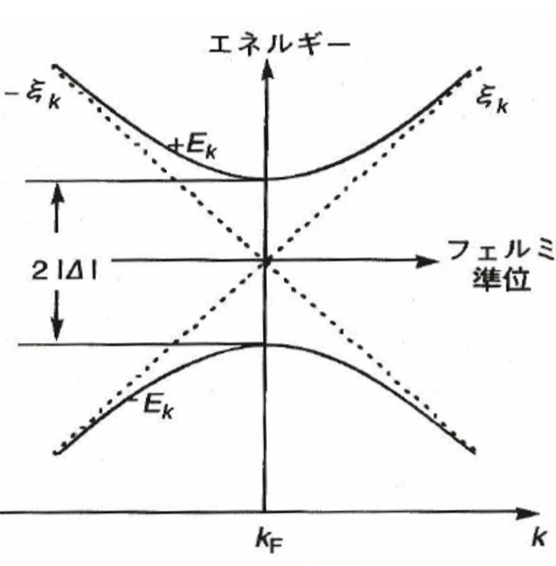
\includegraphics[width=8cm]{Figure/6.png}
\caption{Relation between $E_{k}$ and $\varepsilon_{k}$(Solid line-quasiparticles,Dash line-normal electrons)}
\end{figure}
\begin{solution}
As shown in \textbf{Figure 5}, for quasiparticles, it's $E_{k}$ is a hyperbola function to $\varepsilon_{k}$, while for normal electrons, 
$\Delta_{k}$ is 0, so $E_{k}$ has linear relation with $\varepsilon_{k}$.
\end{solution}

\newpage    
\question We wish to derive the corresponding (2-dimensional) eigenvectors $U^{+}$ and $U^{-}$
In the first case, we can write :
\begin{align*}
U^{+}=\left(\begin{array}{c}
u_{k} \\
v_{k}
\end{array}\right)    
\end{align*}\\
After some algebra, you should be able to find the standard amplitude functions : $u_{k}$ and $v_{k}$, having the property $u_{k}^{2}+v_{k}^{2}=1$.
\begin{solution}
We know $\tilde {\Lambda}$ can diagonalize $H_{eff}$\\
\begin{align*}
H_{e f f} \stackrel{\tilde {\Lambda} }{\Rightarrow }\left(\begin{array}{cc}
+\sqrt{\varepsilon_{k}^{2}+\Delta_{k}^{2}} & 0 \\ 0 & -\sqrt{\Delta_{k}^{2}+\varepsilon_{k}^{2}}
\end{array}\right)      
\end{align*}
$\tilde {\Lambda}$ can be generated by two eigenvectors, to get them, we employ again the eignfunction:
\begin{align*}
\left(\begin{array}{cc}
E_{k}-\varepsilon_{k} & \Delta_{ k} \\
\Delta^{*}_{k} & E_{k}+\varepsilon_{k}
\end{array}\right)\left(\begin{array}{c}
u_{k} \\v_{k}
\end{array}\right)=0 \\
\left(E_{k}-\varepsilon _{k}\right) u_{k}+\Delta_{k} v_{k}=0 \\
\Delta_{k}^{*} u_{k}+\left(E_{k}+\varepsilon _{k}\right) v_{k}=0 \\
u_{k}^{2}+v_{k}^{2}=1
\end{align*}
Then we can get $U^{+}$:
First, we have:
\begin{align*}
\frac{v_{\mathbf{k}}}{u_{\mathbf{k}}}=\frac{\sqrt{\varepsilon _{\mathbf{k}}^{2}+\left|\Delta_{\mathbf{k}}\right|^{2}}-\varepsilon_{\mathbf{k}}}{-\Delta_{\mathbf{k}}^{*}}  
\end{align*}
Then, with $u_{k}^{2}+v_{k}^{2}=1$,
\begin{align*}
\left|u_{\mathbf{k}}\right|^{2}&= \frac{1}{1+\left|\frac{v_{\mathbf{k}}}{u_{\mathbf{k}}}\right|^{2}}=\frac{1}{2} \frac{\left|\Delta_{\mathbf{k}}\right|^{2}}{\varepsilon _{\mathbf{k}}^{2}+\left|\Delta_{\mathbf{k}}\right|^{2}-\varepsilon _{\mathbf{k}} \sqrt{\varepsilon _{\mathbf{k}}^{2}+\left|\Delta_{\mathbf{k}}\right|^{2}}} \\
\left|u_{\mathbf{k}}\right|^{2} &=\frac{1}{2} \frac{\left|\Delta_{\mathbf{k}}\right|^{2}\left(\sqrt{\varepsilon _{\mathbf{k}}^{2}+\left|\Delta_{\mathbf{k}}\right|^{2}}+\varepsilon _{\mathbf{k}}\right)}{(\sqrt{\varepsilon _{\mathbf{k}}^{2}+\left|\Delta_{\mathbf{k}}\right|^{2}})\left(\varepsilon _{\mathbf{k}}^{2}+\left|\Delta_{\mathbf{k}}\right|^{2}-\varepsilon _{\mathbf{k}}^{2}\right)} 
\end{align*}
\begin{align*}
\left|u_{\mathbf{k}}\right|^{2} &=\frac{1}{2}\left(1+\frac{\varepsilon _{\mathbf{k}}}{\sqrt{\varepsilon _{\mathbf{k}}^{2}+\left|\Delta_{\mathbf{k}}\right|^{2}}}\right)=\frac{1}{2}\left(1+\frac{\varepsilon _{\mathbf{k}}}{E_{k}}\right)\\
\left|v_{\mathbf{k}}\right|^{2}&=\frac{1}{2}\left(1-\frac{\varepsilon _{\mathbf{k}}}{\sqrt{\varepsilon _{\mathbf{k}}^{2}+\left|\Delta_{\mathbf{k}}\right|^{2}}}\right)=\frac{1}{2}\left(1-\frac{\varepsilon _{\mathbf{k}}}{E_{k}}\right)
\end{align*}
These are the amplitude functions.
\end{solution}


\question Express the 2 $\times$ 2 transformation matrix $\tilde{\Lambda}=\left(U^{+}, U^{-}\right)$
\begin{solution}
For another eigenvalue $E^{-}$ , the eigenvector is $\left(\begin{array}{c}
-v_{k} \\u_{k}
\end{array}\right)$
So the transform matrix $\tilde{\Lambda}=\left(U^{+}, U^{-}\right)$ is:
\begin{align*}
\tilde{\Lambda}=\left(\begin{array}{cc}
u_{k} & -v_{ k} \\
v_{k} & u_{k}
\end{array}\right)   
\end{align*}
\end{solution}

\question Using  $\tilde{\Lambda}$  find the new  QP  operators  $\gamma_{k}^{+}$  and  $\gamma_{k}^{-}$  in terms of  $a_{k \uparrow}$  and  $a_{-k \downarrow}^{\dagger}$.  Please give a physical interpretation of the quantities:  $\gamma_{k}^{\pm}$, $u_{k}$,  and  $v_{k}$ 
\begin{solution}
\begin{align*}
\tilde{\gamma}_{k}=\left(\begin{array}{l}
\gamma _{k}^{+} \\
\gamma_{k}^{-}
\end{array}\right)=\Lambda \tilde a_{k}=\Lambda\left(\begin{array}{c}
a_{k,\uparrow }  \\
a_{-k,\downarrow }^{*}
\end{array}\right)=\left(\begin{array}{cc}
u_{k} & -v_{k} \\
v_{k} & u_{k}
\end{array}\right)\left(\begin{array}{c}
a_{k,\uparrow }  \\
a_{-k,\downarrow }^{*}
\end{array}\right)
\end{align*}
So,
\begin{align*}
\begin{array}{l}
\gamma_{k}^{+}=u_{k}a_{k,\uparrow } -v_{k} a_{-k ,\downarrow }^{*} \\
\gamma _{k}^{-}=v_{k} a_{k,\uparrow }+u_{k} a_{-k,\downarrow } ^{*}
\end{array}
\end{align*}
The physicsl meaning of $\gamma_{k}^{+}$ and $\gamma_{k}^{-}$ is the creation and annihilation operators of quasiparticles, $a_{-k ,\downarrow }^{*}$ and $a_{k,\uparrow }$ are creation operators of electrons and holes.\\
From previous result describing the behavior of  $u_{\mathbf{k}}$  and  $v_{\mathbf{k}}$,  we have that as  $\Delta_{\mathbf{k}} \rightarrow 0$,$\left|u_{\mathbf{k}}\right|^{2} \rightarrow 1$  for  $\varepsilon_{\mathbf{k}}>0$  and  $\left|u_{\mathbf{k}}\right|^{2} \rightarrow 0$  for  $\varepsilon_{\mathbf{k}}<0 $ whereas  $\left|v_{\mathbf{k}}\right|^{2} \rightarrow 1$  for  $\varepsilon_{\mathbf{k}}<0$  and  $\left|v_{\mathbf{k}}\right|^{2} \rightarrow 0$  for  $\varepsilon_{\mathbf{k}}>0$. 
So $u_{\mathbf{k}}^{2}$  and  $v_{\mathbf{k}}^{2}$ correspond to possibility to find holes and electrons.\\
At the superconducting state, a quasiparticle is a superposition of both an
electron and a hole state. And $u_{k}$ corresponds to the amplitude of hole and $v_{k}$ the amplitude of electron.\\
\begin{align*}
\end{align*}
\textbf{Backup}\\
In other text books, I found they call $\gamma_{\mathbf{k} \sigma}^{\dagger}$ Bogoliubons and correspond to the excitation of quasiparticle.\\
In that book, it also mentioned:\\
\textbf{At the normal state, creating a quasiparticle corresponds to creating an electron for energies above
the Fermi level and creating a hole (destroying an electron) of opposite momentum and spin for energies
below the Fermi level.} \\
But from my equations, this process seemed to corresponds to $\gamma^{-}$ , so I am a little confused.
\end{solution}

\question The figure below shows the  $d I / d V$  measurement as a function of the voltage  V  for a niobium-vacuum-gold $tunneling \quad junction$. The critical temperature of niobium is known to be 9.3 Kelvin. Does the theory (black line) agree well with the experiment (circular dots)? Please explain the key points in a few
sentences.
\begin{figure}[h]
\centering
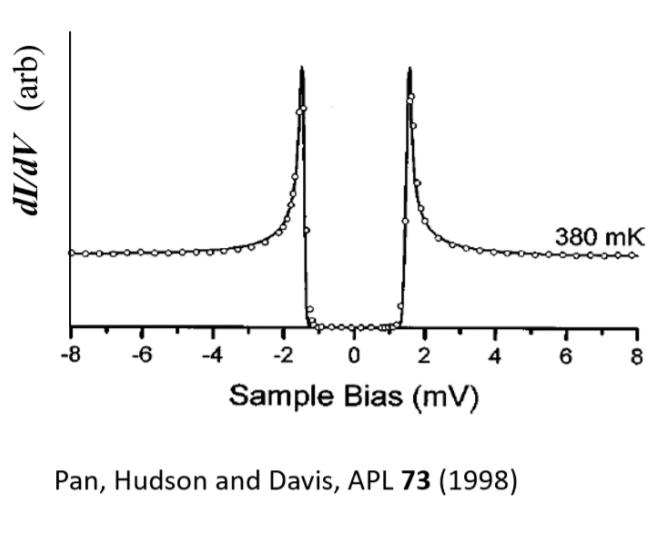
\includegraphics[width=8cm]{Figure/5.png}
\caption{$dI/dV$ of Nb tip-Au }
\end{figure}
\begin{solution}
Yes, they agree very well. And it indicates a superconducting quasiparticle DOS at the Nb-tip end. So we can see the gap clearly.
\end{solution}

\end{questions}

\end{document}